\chapter{Load Testing}
\label{ch:stresstesting}
Si è testata la capacità del sistema di offrire funzionalità senza interruzioni all'aumentare del carico. 
Si è optato per effettuare\textit{ load test} su backend tramite una \textit{suite di test} JMeter. \cite{JMETER}

\section{Implementazione}

I test sono stati impostati per effettuare automaticamente la procedura di login per poi usare \textit{l'access token} così ottenuto per autenticare le richieste inviate verso il backend.

Sono stati simulati 250 utenti concorrenti emettenti richieste a endpoint che prevedono l'uso di \textit{cache}, ripetendo test con lifetime variabili delle \textit{entry} in cache.
La dimensione della tabella di cache è stata mantenuta costante (60000 entry) generando casualmente valori di header \textit{AULOS-hash} (Ch. \ref{ch:caching}).
Il corpo delle richieste è stato fornito tramite un file .csv contenente tutte le possibili richieste generabili da un utente tramite la dashboard.

Testando la performance del backend quando sottoposto a un carico molto superiore a quello previsto dal caso d'uso dell'applicativo, è possibile avere un certo grado di sicurezza che il sistema sarà stabile una volta in utilizzo.

\section{Risultati}
Sono stati eseguiti test senza cache e con \textit{lifetime} di entry in cache pari a 5, 15, 30 e 120 secondi. 
Una volta eseguiti tutti i test, si sono raccolte le seguenti statistiche, divise per durata delle entry di cache. Tutti i test hanno avuto la durata di un'ora.
L'\textit{hit ratio} di entry in cache è stato calcolato secondo la seguente formula, dove x è il prodotto tra lifetime delle entry in cache e \textit{throughput finale} (richieste/s) restituito da JMeter.
\begin{figure}[h!]

\begin{Large}
  \[
    f(x) = \left\{\begin{array}{lr}
        \frac{f(x-1)+\frac{cachesize - f(x-1)}{cachesize}}{cachesize}, & \text{ for } x\geq 1\\
        1 & \text{for } x=0
        \end{array}\right\} = \text{Cache hit ratio}
  \]
\caption{Cache hit ratio formula}
\label{fig:formula}
\end{Large}

\end{figure}
\FloatBarrier
%La figura~\ref{fig:throughput} rappresenta i dati relativi alle richieste al secondo mentre la figura~\ref{fig:hitratio} rappresenta la percentuale stimata di hit in cache durante il test, calcolata tramite la formula in fig.~\ref{fig:formula}.

Di seguito si hanno gli istogrammi ricavati dai dati estrapolati dai test JMeter: 
\begin{figure}[hbpt!]
\caption{Test throughput}
\label{fig:throughput}
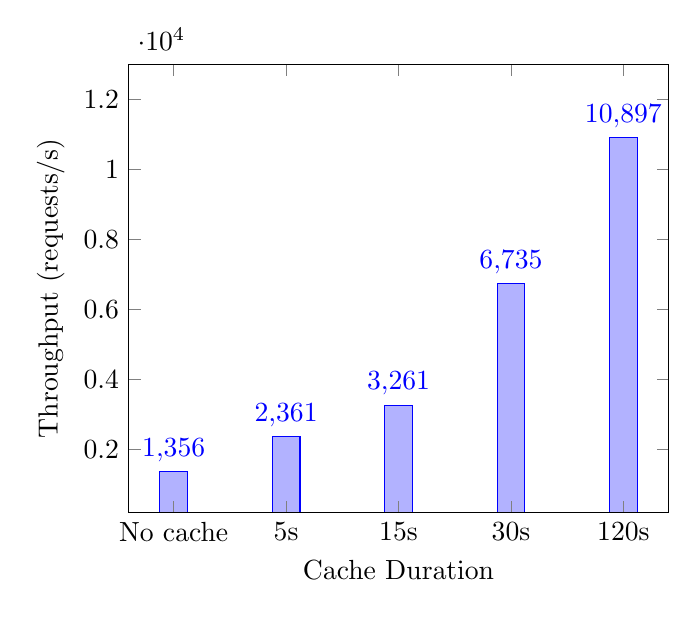
\begin{tikzpicture}
\begin{axis}[  
    hist/symbolic coords={No cache, 5s, 15s, 30s, 120s},
    area style,
    nodes near coords,
    ymax=13000,
    xlabel={Cache Duration},
    ylabel={Throughput (requests/s)}
    ]
\addplot+[ybar, mark=no] plot coordinates { (No cache, 1356) (5s, 2361) (15s, 3261) (30s, 6735) (120s, 10897) };
\end{axis}
\end{tikzpicture}

\end{figure}
\FloatBarrier

In figura~\ref{fig:throughput} si hanno i dati relativi al throughput, sotto forma di richieste soddisfatte con successo al secondo, raggiunto durante i test, organizzati in base alla durata delle entry di cache se attiva.
I dati sono conformi alle aspettative, in quanto è prevedibile che, se soddisfare una richiesta in cache è meno dispendioso del generare dati aggiornati, si abbia un aumento della capacità di soddisfare richieste da parte del backend al diminuire della complessità delle richieste.



\begin{figure}[h!]

\caption{Cache hit ratio}
\label{fig:hitratio}
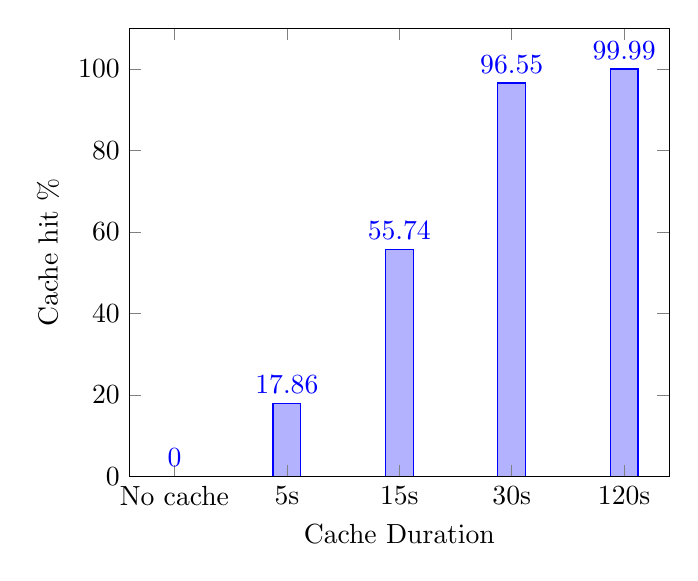
\begin{tikzpicture}
\begin{axis}[
    hist/symbolic coords={No cache, 5s, 15s, 30s, 120s},
    area style,
    nodes near coords,
    ymin=0, ymax=110,
    xlabel={Cache Duration},
    ylabel={Cache hit \%}
    ]
\addplot+[ybar, mark=no] plot coordinates { (No cache, 0) (5s, 17.86) (15s, 55.74) (30s, 96.55) (120s, 99.99) };
\end{axis}
\end{tikzpicture}

\end{figure}
\FloatBarrier
In figura~\ref{fig:hitratio} si ha una stima dell'\textit{hit ratio} in cache, il rapporto tra \textit{cache hit} e richieste totali, calcolato tramite la formula~\ref{fig:formula}, che rappresenta una stima delle entry occupate in cache dopo un numero \emph{x} richieste soddisfatte dato un numero di richieste abilitate alla registrazione in cache fisso con pari probabilità di essere lanciate.

Chiaramente, questo calcolo sarebbe completamente inutile in un contesto reale, in quanto sarebbe ingenuo considerare finito il numero di richieste possibili senza una conoscenza assoluta di ogni livello del contesto applicativo: durante il testing, era infatti nota la possibilità di generare solamente circa 2500 richieste univoche utilizzando il \textit{dataset} a disposizione durante lo sviluppo.

